\chapter{Results}
\label{sec:result}
\section{Results on English Datasets}

\begin {table}[H]
\centering
\begin{tabular}{ | c | c | }
\hline
\textbf{Method} & \textbf{Accuracy} \\ \hline
Maas et al.(2011) & 88.89\\ \hline
NBSVM-bi (Wang \& Manning, 2012) & 91.22\\ \hline
NBSVM-uni (Wang \& Manning, 2012) & 88.29\\ \hline
SVM-uni (Wang \& Manning, 2012) & 89.16\\ \hline
Paragraph Vector (Le and Mikolov(2014)) & 92.58\\ \hline
WordVector+Wiki(Our Method) & 88.60\\ \hline
WordVector+TfIdf(Our Method) & 89.03\\ \hline
WordVector Averaging+TfIdf+Document Vector & \textbf{93.91}\\ \hline

\end{tabular}
\caption {Results on IMDB Movie Review Dataset}
\label{table:IMDB}
\end{table}

Table \ref{table:IMDB} summarizes the results obtained by others and by us on the IMDB movie review dataset. We have gone above the previous best(\cite{Le:14}) by a margin of 1.33\% using enhanced document vector.

\begin {table}[H]
\centering
\begin{tabular}{ | c | c | }
\hline
\textbf{Method} & \textbf{Accuracy} \\ \hline
WordVector Averaging+TfIdf+Document Vector & 93.91\\ \hline
WordVector+TfIdf+Document Vector+RNNLM(Our Method) & \textbf{94.19}\\ \hline
\end{tabular}
\caption {Results on IMDB Movie Review Dataset}
\label{table:IMDB_rnnlm}
\end{table}

The main contributor for improvement in results is our enhanced document vector which overcomes the weaknesses of BOW and document vectors taken separately.\\
Table \ref{table:IMDB_rnnlm} is a further improvement in results once we incorporate predictions of RNNLM and enhanced document vector model together(voting ensemble).

\begin {table}[H]
\centering
\begin{tabular}{ | c | c | }
\hline
\textbf{Method} & \textbf{Accuracy} \\ \hline
WordVector Averaging & 88.42\\ \hline
Weighted WordVector Average & 88.41\\ \hline
WordVector Averaging+Wiki & 88.60\\ \hline
WordVector Averaging+TfIdf & 89.03\\ \hline
WordVector Averaging+Document Vector & 93.24\\ \hline
WordVector Averaging+Wiki+Document Vector & 93.18\\ \hline
WordVector Averaging+Document Vector+RNNLM & 93.70\\ \hline
WordVector Averaging+Wiki+Document Vector+RNNLM & 93.57\\ \hline
WordVector Averaging+TfIdf+Document Vector & 93.91\\ \hline
WordVector Averaging+Wiki+Document Vector+TfIdf & 93.55\\ \hline
WordVector Averaging+TfIdf+Document Vector+RNNLM & \textbf{94.19}\\ \hline
\end{tabular}
\caption {Comparison of results on IMDB Movie Review Dataset with Various Features}
\label{table:IMDB_features}
\end{table}

\begin{figure}[H]
\centering
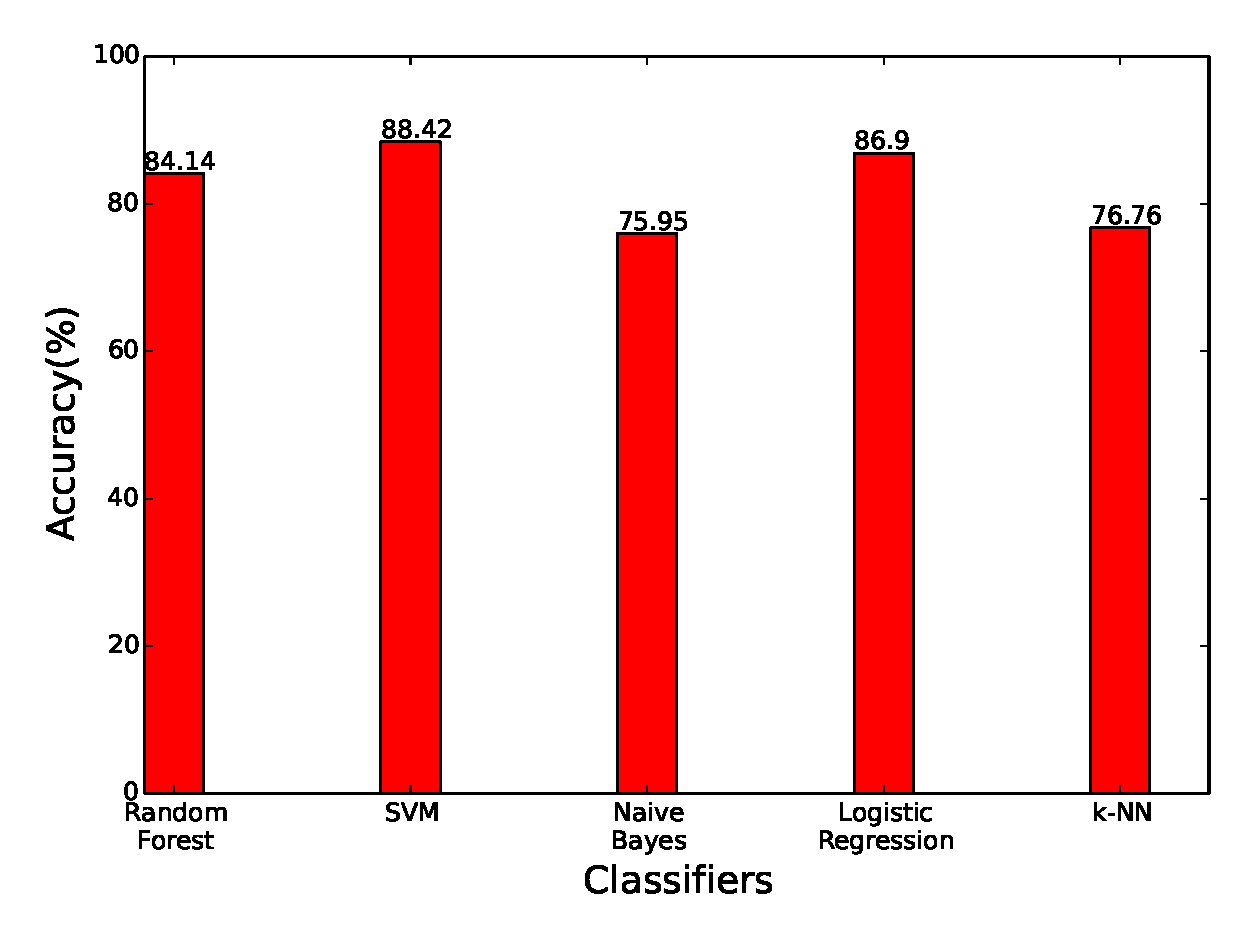
\includegraphics[width=140mm, height=120mm]{accuracy_wordvectors.eps}
\caption{Accuracies of Different Classifiers with Average Word Vectors(IMDB). \label{fig:accuracy_wordvectors}}
\end{figure}

Table \ref{table:IMDB_features} gives an overview of the results obtained with various experiments that we conducted on IMDB dataset. We have tried various vector composition models and feature composition models to obtain good results. Even a simple feature composition of word and document vector yield an improvement over the existing state-of-the-art suggesting that feature composition is a vital area when it comes to NLP tasks such as sentiment analysis.

Figure \ref{fig:accuracy_wordvectors} gives an overview of accuracies of various classifiers using word vector averaging method on IMDB dataset. This clearly gives a green signal to us for using Linear SVM as our classier in all experiments.



Table \ref{table:amazon} presents result of another experiment conducted on famous Amazon electronics review dataset(refer \ref{data:amazon}). Our vector averaging method alone has beaten previous best by 3.3\% which was based on maximum entropy method.
\begin {table}[H]
\centering
\begin{tabular}{ | c | c | }
\hline
\textbf{Features} & \textbf{Accuracy} \\ \hline
Dredze et al.(2008) & 85.90\\ \hline
Max Entropy & 83.79\\ \hline
WordVector Averaging (Our Method) & 89.41\\ \hline
WordVector Averaging+Document Vector(Our Method) & \textbf{92.17}\\ \hline
\end{tabular}
\caption {Results on Amazon Electronics Review Dataset}
\label{table:amazon}
\end{table}


\section{Results on Hindi Datasets}
\label{sec:hindi_results}
\begin {table}[h!]
\centering
\begin{tabular}{ | c | c | c | }
\hline
\textbf{Features} & \textbf{Accuracy(1)} & \textbf{Accuracy(2)} \\ \hline
WordVector Averaging & 78.0 & 79.62\\ \hline
WordVector+tf-idf & 90.73 & 89.52\\ \hline
WordVector+tf-idf without stop words & 91.14 & 89.97\\ \hline
Weighted WordVector & 89.71 & 85.90\\ \hline
Weighted WordVector+tf-idf & \textbf{92.89} & \textbf{90.30}\\ \hline
\end{tabular}
\caption {Accuracies for Product Review and Movie Review Datasets.}
\label{table:hindi_ourmethods}
\end{table}

Table \ref{table:hindi_ourmethods} represents the results using five different techniques for feature set construction. We see that there is a slight improvement in accuracy on both datasets once we remove stop-words but the major breakthrough occurs once we used weighted averaging technique for construction of document vectors from word vectors.

\begin {table}[h!]
\centering
\begin{tabular}{ | c | c | c | }
\hline
\textbf{Experiment} & \textbf{Features} & \textbf{Accuracy} \\ \hline
Subjective Lexicon (Bakliwal et al.(2012)) & Simple Scoring & 79.03\\ \hline
Hindi-SWN Baseline (Arora et al.(2013)) & Adjective and Adverb presence & 69.30\\ \hline
Word Vector with SVM (Our method) & tf-idf with word vector & 91.14\\ \hline
Weighted Word Vector with SVM (Our method) & tf-idf+weighted word vector & \textbf{92.89}\\ \hline
\end{tabular}
\caption {Comparison of Approaches: Product Review Dataset}
\label{table:hindi_product}
\end{table}
Table \ref{table:hindi_product} and \ref{table:hindi_movie} compares our best method with various other methods which have performed well using techniques such as \emph{tf-idf}, subjective lexicon, etc.

\begin {table}[h!]
\centering
\begin{tabular}{ | c | c | c | }
\hline
\textbf{Experiment} & \textbf{Features} & \textbf{Accuracy} \\ \hline
In language using SVM (Joshi et al.(2010)) & tf-idf & 78.14\\ \hline
MT Based using SVM (Joshi et al.(2010)) & tf-idf & 65.96\\ \hline
Improved Hindi-SWN  (Bakliwal et al.(2012)) & Adj. and Adv. presence & 79.0\\ \hline
WordVector Averaging & word vector & 78.0\\ \hline
Word Vector with SVM (Our method) & tf-idf; word vector & 89.97\\ \hline
Weighted Word Vector with SVM (Our method) & tf-idf+weighted word vector & \textbf{90.30}\\ \hline
\end{tabular}
\caption {Comparison of Approaches: Movie Review Dataset}
\label{table:hindi_movie}
\end{table}

Table \ref{table:hindi_neighbors} shows the top few similar words for certain words from the corpus with cosine similarity as a distance metric. The words which have higher cosine similarity tend to be semantically and syntactically related.
\begin {table}[ht!]
\centering
\begin{tabular}{ | c | c | c | }
\hline
\textbf{{\dn aQCA}} & \textbf{{\dn{KrAb}}} & \textbf{{\dn ByAnk}} \\ \hline
{\dn b\7{h}t} & {\dn EnrAsAjnk} & {\dn By\306wkr}\\ \hline
{\dn \7{s}pr} & {\dn kM)or} & {\dn BFqZ}\\ \hline
{\dn k\?vl} & {\dn nA\7{)}k} & {\dn ByAvh}\\ \hline
{\dn itnA} & {\dn bdtr} & {\dn avsAd}\\ \hline
\end{tabular}
\caption {Some sentiment words and their neighbors}
\label{table:hindi_neighbors}
\end{table}

\section{Odd One Out}
We trained Skip-Gram model on latest English and Hindi Wikipedia dump and tried to analyze the quality of embeddings by finding the odd word amongst a list of words. For this task, we took found cosine similarity between each pair and found the word with lowest cosine similarity with every other. The results are highlighted below-

\begin{table}[ht!]
\centering
\Large
\begin{tabular}{|l|l|l|l|}
\hline
breakfast         & \textbf{cereal} & lunch        & dinner  \\ \hline 
eight             & seven           & \textbf{owe} & nine    \\ \hline 
\textbf{shopping} & math            & reading      & science \\ \hline
\end{tabular}
\caption{Odd One Out in English}
\label{fig:english_odd}
\end{table}

\begin{table}[ht!]
\centering
\Large
\begin{tabular}{|l|l|l|l|}
\hline
{\dn BArt} & \textbf{{\dn \7{m}MbI}} & {\dn !s} & {\dn cFn}  \\ \hline 
{\dn lwkF}  & {\dn b\?hn} & \textbf{{\dn md\0}} & {\dn mEhlA}    \\ \hline 
\textbf{{\dn u\38Dwog}} & {\dn n\?tA}  & {\dn m\2/F} & {\dn srkAr} \\ \hline
\end{tabular}
\caption{Odd One Out in Hindi}
\label{fig:hindi_odd}
\end{table}

\section{Similar Words}
The trained skip-gram model was used for this task as well. We found the top few words which were closer in terms of cosine distance to the give word. The results are highlighted below-
\begin{table}[ht!]
\centering
\large
\begin{tabular}{|l|l|l|l|l|}
\hline
\textcolor{blue}{\textbf{Father}} & \textcolor{blue}{\textbf{France}} & \textcolor{blue}{\textbf{XBOX}} & \textcolor{blue}{\textbf{scratched}} & \textcolor{blue}{\textbf{megabits}} \\ \hline
grandfather & Germany & XBLA  & scraped & gigabits  \\ \hline 
uncle & French & Xbox360  & rubbed & kilobits  \\ \hline 
mother & Greece & SmartGlass  & bruised & megabit  \\ \hline 
father-in-law & Netherlands & 360/PS3  & cracked & terabits  \\ \hline 
brother & Scotland & XBLA   & discarded & MB/s  \\ \hline 
- & - & Qubed  & shoved & Tbit/s  \\ \hline 
- & - & Kinect  & tripped & -  \\ \hline 
\end{tabular}
\caption{Top Few Similar words in English}
\label{fig:english_similar}
\end{table}

\begin{table}[ht!]
\centering
\large
\begin{tabular}{|l|l|l|}
\hline
\textcolor{blue}{\textbf{{\dn BArt}}} & \textcolor{blue}{\textbf{{\dn \326wyApAr}}} & \textcolor{blue}{\textbf{{\dn aobAmA}}} \\ \hline
{\dn \3FEwd\?f} & {\dn \326wyvsAy} & {\dn E\3CAw\2Vn}  \\ \hline 
{\dn Et\3A9wt} & {\dn \7{p}nbF{\qvb}mA} & {\dn brAk} \\ \hline 
{\dn d\?f} & {\dn vAEZ>y} & {\dn sFn\?Vr} \\ \hline 
{\dn aA\1D\5\3FEwd\?f} & {\dn b\4{\qva}Ek\2g} & {\dn rA\6{\3A3w}pEt} \\ \hline 
{\dn l\38CwAK} & {\dn u\38Dwog} & {\dn uMmFdvAr} \\ \hline 
\end{tabular}
\caption{Top Few Similar words in Hindi}
\label{fig:hindi_similar}
\end{table}
